\documentclass[]{article}
\usepackage{amsmath}
\usepackage{amsthm}
\usepackage{amssymb}
\usepackage{ulem}
\usepackage{graphicx}
\usepackage{tikz}
\usetikzlibrary{matrix,shapes,arrows,positioning,chains}
\usepackage{tkz-base}
\usepackage{tkz-euclide}
\usepackage
[
left=2cm,
right=2cm,
top=2cm,
bottom=2cm,
]
{geometry}

\begin{document}

\newtheorem{problem}{Problem}
\newtheorem{lemma}{Property}

\section{The binary search problem, and its variation}

Here is a git repository of a software. It is known that somewhere in the recent N commits, a bug was introduced, and the task is to efficiently find the commit that introduced the bug.

A well-known solution is to use \texttt{git bash}, i.e. the binary search method: checking the commit at the middle of the commit list, and then depending on the result, checking the commit at the middle of one half parts of the commit list. This is the fastest method under normal conditions.

Now we make a small change to the problem: if the commit to check contains the bug (i.e. it is or is after the first commit introducing the bug), the software would crash the entire computer system during the test and the test has to reboot the computer, which takes five minutes. Testing a software without the bug still takes a short time, say, 30 seconds. In this case, what is the best way to implement the binary search?

One might want to test more "good" commits to avoid time spent on "bad" commits as much as possible. Therefore he would tend to test commits before the middle commit, resulting a test sequence "biased" towards the older commits. In an extreme case, where the bad commits take forever to test, he would just test commits one by one from the oldest commit, until he finds the first commit that crashes the system. Similarly, if a bad commit actually takes less time to test, the binary search would bias towards the newer commits.

Under these conditions, the question is, using the binary search idea, what would be the best commit to test in order to minimize the time cost?

\section{Mathematical formalization}

Let's formalize the question in mathematical languages:

\begin{problem}
	Given a sequence $a_0, a_1, a_2, ..., a_n$, with a number $j$ such that $a_k = 0, \forall k < j$ and $a_k = 1, \forall k \ge j$. $j$ is a random number evenly distributed among integers $1, 2, ..., n$. To get the value of $a_k$, some time is taken. The time cost is $s$ if $a_k = 0$, or $t$ if $a_k = 1$. What is the best method to find $j$ with minimal expectation of total time cost?
\end{problem}

and with some assumption clarified:
\begin{itemize}
	\item The values $a_0 = 0$ and $a_n = 1$ are already known and no need to test. Their existence in the problem is to simplify the numbering system in the solution.
	\item Testing cannot be done in parallel. One cannot start another test until the previous test is finished.
	\item Only testing takes time. Other step is assumed done instantly.
	\item One may get the result by noticing one test takes a longer time before producing the result. However, getting the result in advance does not shorter the time taken by the test, not even for the final step. The total time cost includes the final "rebooting" time even if one already knows the answer.
\end{itemize}

\section{Testing procedure}

The binary-search-like method is illustrated in the chart below.

\tikzstyle{decision} = [diamond, draw, fill=blue!20, 
text width=4.5em, text badly centered, node distance=3cm, inner sep=0pt]
\tikzstyle{block} = [rectangle, draw, fill=blue!20, 
text width=5em, text centered, minimum height=4em, node distance=3cm]
\tikzstyle{line} = [draw, -latex']
\tikzstyle{cloud} = [draw, ellipse,fill=red!20, node distance=2cm,
minimum height=2em]

\begin{tikzpicture}[auto]
\node [cloud](start){start};
\node [block, below of=start](init){set $p = 0$, $q = n$};
\node [decision, below of=init](exit){$p - q = 1$?};
\node [block, below of=exit](choose){$(*)$choose integer $x$ such that $p < x < q$};
\node [decision, below of=choose](test){test $a_x$};
\node [block, left of=test](a){set $p=x$};
\node [block, right of=test](b){set $q=x$};
\node [block, right of=exit](final){set $j=q$};
\node [cloud, below of=final](end){end};

\path [line] (start) -- (init);
\path [line] (init) -- (exit);
\path [line] (exit) -- node {no} (choose);
\path [line] (choose) -- (test);
\path [line] (test) -- node {0, $+s$} (a);
\path [line] (test) -- node {1, $+t$} (b);
\path [line] (a) |-([xshift=-0.5cm,yshift=-0.5cm]a.south west)|- (exit);
\path [line] (b) |-([xshift=-0.5cm,yshift=-0.5cm]a.south west)|- (exit);
\path [line] (exit) -- node{yes} (final);
\path [line] (final) -- (end);

\end{tikzpicture}

\section{The equation}
 
The step $(*)$ is the only place we need to decide how to do exactly. It can be seen that on each iteration, the algorithm is effectively solving the same problem with a smaller size where $n = p - q$, therefore we can choose x by some function $w_{s,t}(n)$ as
\[
x = w_{s,t}(p - q) + p \,,
\]
and the expectation of total time $F_{s,t}(n)$ can be expressed recursively as
\begin{equation}
F_{s,t}(n) = \frac{w}{n}(t + F_{s,t}(w)) + \frac{n-w}{n}(s + F_{s,t}(n-w))\,,
\end{equation}
where $w = w_{s,t}(n)$ represents the offset of the next testing point relative to the start of the current range. The two term represents the two possibility where the next iteration goes to the left or the right. Their probability are $\frac{w}{n}$ and $\frac{n-w}{n}$, respectively, based on the assumption of the uniform distribution. $t$ and $s$ are the time cost of the current iteration, and $F(...)$ are the time cost of the rest iteration.

Our goal is to find the most efficient method, so we want to minimize the value of $F(n)$. Therefore, with an initial value $F(1) = 0$, we can define a calculable function $F(n)$ over $n \in \mathbb{Z}$ as
\begin{align*}
F_{s,t}(1) &= 0\,,\\
F_{s,t}(n) &= \min_{0<w<n}^{w\in\mathbb{Z}}\left\{\frac{w}{n}(t + F_{s,t}(w)) + \frac{n-w}{n}(s + F_{s,t}(n-w))\right\} \textrm{ for } n > 1 \,.
\end{align*}

To simplify further analysis, we define the ``normalized" function $E(n) = nF(n)$, which satisfies the following recursive relation
\begin{align*}
E_{s,t}(1) &= 0\,,\\
D^{w}_{s,t}(n) &= E_{s,t}(w) + E_{s,t}(n-w) + wt +(n-w)s,&\textrm{ for } n > 1, w=1,2,\dots,n-1, \\
E_{s,t}(n) &= \min_{0<w<n}^{w\in\mathbb{Z}}\{D^{w}_{s,t}(n)\} = D^{w_{s,t}(n)}_{s,t}(n) &\textrm{ for } n > 1 \,.
\end{align*}

Now let's analyze the function $E_{s,t}(n)$, which represents the expected time scaled by $n$, and the optimizer $w = w_{s,t}(n)$, which represents which commit you should test next given parameters $(n,s,t)$.

\section{Properties}
\hspace{1cm}
\begin{lemma} Homogeneity of $s$ and $t$. For any $k\in\mathbb{R}^+$ we have
\[
	E_{ks,kt}(n) = k E_{s,t}(n)
\]
\[
	w_{ks,kt}(n) = w_{s,t}(n)
\]
This means it is only the ratio $s/t$ that affects the bisecting strategy.
\end{lemma}
\begin{proof}
		Proof by induction. 
	\paragraph{Base case} for $n = 1$, $E_{ks,kt}(1) = 0 = k\cdot0 = kE_{s,t}(1)$
	\paragraph{Inductive step} Assuming $E_{ks,kt}(m) = k E_{s,t}(m)$ holds for all $m = 1,2,\dots,n-1$, we can show that $E_{ks,kt}(n) = k E_{s,t}(n)$ by 
	\begin{align*}
	E_{ks,kt}(n) &= \min_{w}\{E_{ks,kt}(w) + E_{ks,kt}(n-w) + wkt +(n-w)kst\}\\
	  &= \min_{w}\{k E_{s,t}(w) + k E_{s,t}(n-w) + wkt +(n-w)ks\}\\
	  &= k\min_{w}\{E_{s,t}(w) + E_{s,t}(n-w) + wt +(n-w)s\}\\
	  &=kE_{s,t}(n)
	\end{align*}
	and note that the transformation doesn't affect the choice of $w$.
\end{proof}	

\hspace{1cm}
\begin{lemma} Symmetry of $s$ and $t$:
	\[
		E_{s,t}(n) = E_{t,s}(n)
	\]
	\[
		w_{s,t}(n) + w_{t,s}(n) = n
	\]
Together with previous lemma, this means we only needs to study either $s/t \le1$ or $s/t \ge 1$
\end{lemma}
\begin{proof}
	This can be similarly proved by induction. Omitted.
\end{proof}	

\hspace{1cm}
\begin{lemma}
	The optimizer $w_{s,t}(n)$ outputs a set of $w$. It is not necessarily always a single $w$ that minimize the function
\end{lemma}
\begin{proof}
		This is obvious. We haven't really restricted $w$ to be a single value for given $(n,s,t)$. Multiple $w$ can equally give the minimal result in the $E_{s,t}(n)$ equation. In fact, we will see that this is true for most cases. 
\end{proof}	

\hspace{1cm}
\begin{lemma}
$E_{s,t}(n)$ as a function of $n$ is convex
\end{lemma}
\begin{lemma}
	$w_{s,t}(n)$ is always a simple integer interval $[w_{s,t}^{min}(n), w_{s,t}^{max}(n)]$
\end{lemma}
\begin{lemma}
	If $w^*\in w_{s,t}(n)$, then at least one of the following is true: $w^*\in w_{s,t}(n+1)$, or $w^*+1\in w_{s,t}(n+1)$
\end{lemma}
\begin{proof}
(TODO, currently broken)
we will prove the three properties above together using induction.

First of all, let's formally define the convexity of $E(n)$ which is a discrete function over integer. We define the differential as
\[  
\Delta E(n) = E(n+1) - E(n)
\]
and we say that $E_{s,t}(n)$ is convex on $[1,n]$ if and only if
\[
 \Delta E(m)\le \Delta E(m+1)\quad\forall m = 1,2,\dots,n-2\quad (\text{Proposition } \mathbf{C}_n)
\]

We denote the property about $w$ as
\[
w^*\in w(n) \implies w^* \in w(n+1) \lor w^*+1 \in w(n+1) \quad (\text{Proposition } \mathbf{W}_n)
\]

We also denote $D^w_{s,t}(n) = E_{s,t}(w) + E_{s,t}(n-w) +wt+(n-w)s$ so we have
\[
E(n) = \min_w\{D^w(n)\} = D^{w(n)}(n)
\]
\[
D^{w(n)}(n) \le D^{w(n) - 1}(n)\  (\text{if } w(n) > 1)
\]
\[
D^{w(n)}(n) \le D^{w(n) + 1}(n)\  (\text{if } w(n) < n - 1)
\]
We also have 
\[
D^{w}(n+1) = D^{w} + \Delta E(n-w) +s
\]
\[
D^{w+1}(n+1) = D^{w} + \Delta E(w) +t
\]


\paragraph{Base case}
The first few values of $E(n)$ and $w(n)$ are 
\begin{align*}
&E(1) = 0,\ &&\\
&E(2) = s + t, \ &&w(2) = 1,\\
&E(3) = 2s + 2t + \min\{s, t\}, \ &&w(3) = \{1\}, \{2\},\text{ or }\{1,2\}
\end{align*}
It can be seen that proposition $\mathbf{C}_1$ and $\mathbf{W}_2$ hold.

\paragraph{Inductive step} (a) we will show that $\mathbf{C}_n \implies \mathbf{W}_n$ for $n\ge 2$:

If $w(n) >1$, then we have
\begin{align*}
D^{w(n)}(n+1) &= D^{w(n)}(n) + \Delta E(n-w(n)) +s\\
&\le  D^{w(n) - 1}(n) + \Delta E(n-w(n)) +s \quad &(\text{$D^{w(n)}(n)$ is the smallest among $D^{w}(n)$})\\
&\le  D^{w(n) - 1}(n) + \Delta E(n-(w(n)-1)) +s \quad &(\text{Convexity $\mathbf{C}_{n}$}) \\ 
&=D^{w(n)-1}(n+1)
\end{align*}

If $w(n) < n -1$, then we have
\begin{align*}
D^{w(n)+1}(n+1) &= D^{w(n)}(n) + \Delta E(w(n)) +t \\
&\le  D^{w(n) + 1}(n) + \Delta E(w(n)) +t \quad &(\text{$D^{w(n)}(n)$ is the smallest among $D^{w}(n)$})\\
&\le  D^{w(n) + 1}(n) + \Delta E(w(n) + 1) +t \quad &(\text{Convexity $\mathbf{C}_{n}$}) \\ 
&= D^{w(n)+2}(n+1)
\end{align*}

Also notice that $D^w(n+1)$ is convex over $w=1,\dots,n$ due to convexity $\mathbf{C}_{n}$. The inequalities above shows the relations about four consecutive points at the valley of the convex function:
\[
D^{w(n)-1}(n+1) \ge D^{w(n)}(n+1) \sim D^{w(n)+1}(n+1) \le D^{w(n)+2}(n+1)
\]

We can conclude that at least one of $D^{w(n)}(n+1)$ or $D^{w(n)+1}(n+1)$ is the minimum of $D^w(n+1)$, thus $\mathbf{W}_n$ holds

(b) We then show that:
\[
\Delta E(n)= \begin{cases}
	\Delta E(w(n)) + t \quad(w(n+1) = w(n) + 1)\\
	\Delta E(n-w(n)) + s\quad(w(n+1) = w(n))
	\end{cases} \quad (\text{Proposition $\mathbf{W}_n$ ehhhhhhhh})
\]

\end{proof}



\hspace{1cm}
\begin{lemma}
Fixing $n$ and $s$, $E_{s,t}(n)$ as a function of $t$ is concave 
\end{lemma}
\begin{proof}
Proof by induction. The base case $E_{s,t}(1) = 0$ is concave over $t$. In the recursive equation, all the summation components are concave, and the minimal of concave functions is still a concave function.
\end{proof}

\hspace{1cm}
\begin{lemma}
Fixing $n$ and $s$, $E_{s,t}(n)$ is a piecewise linear function of $t$. The nodes are always at rational points.
\end{lemma}
\begin{proof}
	This can be proved by induction. Omitted.
\end{proof}
With this property, we can graph the function with a series of segments. For example, the graph of $E_{1,t}(10)$ over $t\in[0,1]$ is 


	\begin{tikzpicture}[scale=0.8]
	\tkzInit[xmin=0,ymin=0,xmax=1.1,ymax=35,xstep=0.1,ystep=5]
	\tkzDrawX[label={$t$}]
	\tkzLabelX[step=1]
	\tkzDrawY[label={$E_{1,t}(10)$}]
	\tkzLabelY[step=10]
	\tkzDefPoint(0,9){p1}
	\tkzDefPoint(1/8,117/8){p2}
	\tkzDefPoint(1/6,97/6){p3}
	\tkzDefPoint(1/5,86/5){p4}
	\tkzDefPoint(1/3,62/3){p5}
	\tkzDefPoint(1/2,49/2){p6}
	\tkzDefPoint(1,34){p7}
	\tkzDefPoint(1.1,35.5){p8}
	\tkzDrawSegment(p1,p2)
	\tkzDrawSegment(p2,p3)
	\tkzDrawSegment(p3,p4)
	\tkzDrawSegment(p4,p5)
	\tkzDrawSegment(p5,p6)
	\tkzDrawSegment(p6,p7)
	\tkzDrawSegment(p7,p8)
	\tkzDrawPoints(p1,p2,p3,p4,p5,p6,p7)
	\tkzLabelPoint[right](p1){\tiny $(0,9)$}
	\tkzLabelPoint[right](p2){\tiny $(1/8,117/8)$}
	\tkzLabelPoint[right](p3){\tiny $(1/6,97/6)$}
	\tkzLabelPoint[right](p4){\tiny $(1/5,86/5)$}
	\tkzLabelPoint[right](p5){\tiny $(1/3,62/3)$}
	\tkzLabelPoint[right](p6){\tiny $(1/2,49/2)$}
	\tkzLabelPoint[right](p7){\tiny $(1,34)$}
	\end{tikzpicture}

We omitted the graph beyond $t=1$, but remember that it can be derived by $E_{1,t}(n) = t\cdot E_{1,1/t}(n)$ due to symmetry and homogeneity.

It can be seen from the graph that nodes are generally at $t = 1/p$ with some integer $p$. This isn't always true for larger $n$, but computation shows that most nodes are at simple ratios like these.

\hspace{1cm}
\begin{lemma}
	Fixing $n$ and $s$, $w_{s,t}(n)$ is a ``piecewise constant" function. Over a single segment of the piecewise function $E_{s,t}(n)$, the same set of $w$ is chosen. However, at node of piecewise function $E_{s,t}(n)$, $w_{s,t}(n)$ can take a unique value that's not equal to either the left segment or the right segment.
\end{lemma}
\begin{proof}
	Remember that $E_{s,t}(n)$ calculated by taking the $t$-pointwise minimum of a sequence of piecewise linear, convex functions $J_w(t) = E_{s,t}(w) + E_{s,t}(n-w) + wt +(n-w)s$ indexed by $w$. If the pointwise minimum results in a simple linear function over an $t$-interval, it must be resulted from the same set of $w$. This is because, if any $J_w(t)$ tries to join or leave $E_{s,t}(n)$ midway in the interval, it must bend down due to convexity, and that would result in  $E_{s,t}(n) \le J_w(t)$ bending down as well, contradicting with the fact that $E_{s,t}(n)$ is a simple linear function in this interval. $J_w(t)$ can only join or leave at the nodes of $E_{s,t}(n)$
\end{proof}

If we graph $w$ over $t$, we will get a series of ``blocks", separated by vertical lines (marked red) at the nodes of $E$ over $t$. For example, the graph of $w_{1,t}(10)$ over $t\in[0,1]$ is 

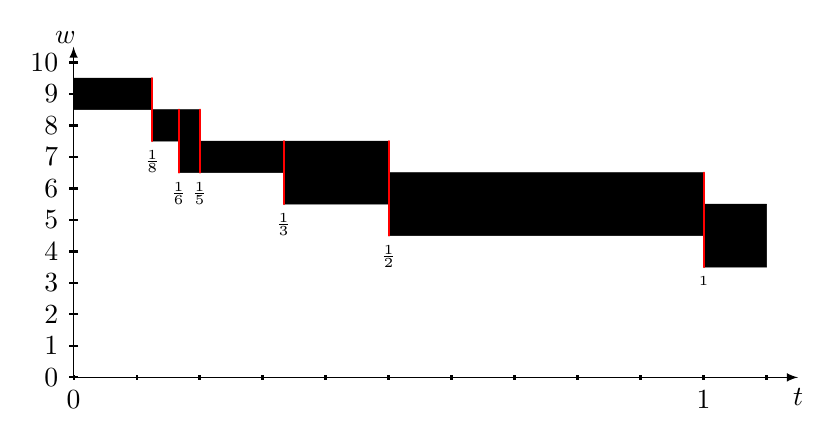
\begin{tikzpicture}[xscale=0.8,yscale=0.4]
\tkzInit[xmin=0,ymin=0,xmax=1.1,ymax=10,xstep=0.1,ystep=1]
\tkzDrawX[label={$t$}]
\tkzLabelX[step=1]
\tkzDrawY[label={$w$},above]
\tkzLabelY[step=1]
\tkzDefPoint(0, 8.5){A}\tkzDefPoint(1/8,9.5){C}\tkzDefRectangle(A,C)\tkzGetPoints{B}{D} \tkzDrawPolygon[fill=black](A,...,D)
\tkzDefPoint(1/8, 7.5){A}\tkzDefPoint(1/6,8.5){C}\tkzDefRectangle(A,C)\tkzGetPoints{B}{D} \tkzDrawPolygon[fill=black](A,...,D)
\tkzDefPoint(1/6, 6.5){A}\tkzDefPoint(1/5,8.5){C}\tkzDefRectangle(A,C)\tkzGetPoints{B}{D} \tkzDrawPolygon[fill=black](A,...,D)
\tkzDefPoint(1/5, 6.5){A}\tkzDefPoint(1/3,7.5){C}\tkzDefRectangle(A,C)\tkzGetPoints{B}{D} \tkzDrawPolygon[fill=black](A,...,D)
\tkzDefPoint(1/3, 5.5){A}\tkzDefPoint(1/2,7.5){C}\tkzDefRectangle(A,C)\tkzGetPoints{B}{D} \tkzDrawPolygon[fill=black](A,...,D)
\tkzDefPoint(1/2, 4.5){A}\tkzDefPoint(1,6.5){C}\tkzDefRectangle(A,C)\tkzGetPoints{B}{D} \tkzDrawPolygon[fill=black](A,...,D)
\tkzDefPoint(1, 3.5){A}\tkzDefPoint(1.1,5.5){C}\tkzDefRectangle(A,C)\tkzGetPoints{B}{D} \tkzDrawPolygon[fill=black](A,...,D)
\tkzDefPoint(1/8, 7.5){A}\tkzDefPoint(1/8,9.5){B}\tkzDrawSegment[color=red,thick](A,B)\tkzLabelPoint[below](A){\tiny $\frac{1}{8}$}
\tkzDefPoint(1/6, 6.5){A}\tkzDefPoint(1/6,8.5){B}\tkzDrawSegment[color=red,thick](A,B)\tkzLabelPoint[below](A){\tiny $\frac{1}{6}$}
\tkzDefPoint(1/5, 6.5){A}\tkzDefPoint(1/5,8.5){B}\tkzDrawSegment[color=red,thick](A,B)\tkzLabelPoint[below](A){\tiny $\frac{1}{5}$}
\tkzDefPoint(1/3, 5.5){A}\tkzDefPoint(1/3,7.5){B}\tkzDrawSegment[color=red,thick](A,B)\tkzLabelPoint[below](A){\tiny $\frac{1}{3}$}
\tkzDefPoint(1/2, 4.5){A}\tkzDefPoint(1/2,7.5){B}\tkzDrawSegment[color=red,thick](A,B)\tkzLabelPoint[below](A){\tiny $\frac{1}{2}$}
\tkzDefPoint(1/1, 3.5){A}\tkzDefPoint(1/1,6.5){B}\tkzDrawSegment[color=red,thick](A,B)\tkzLabelPoint[below](A){\tiny $1$}

\end{tikzpicture}

We omitted the graph beyond $t=1$, but remember that it can be derived by $w_{1,t}(n) = n - w_{1,1/t}(n)$ due to symmetry and homogeneity.

In the case of $n=10$, the vertical lines at nodes don't exceed the $w$ range of its adjacent blocks, but this is not always true for larger $n$. Some vertical lines can looks ``spiky", demonstrating a much larger set of $w$ than the adjacent blocks. This also demonstrates the non-monotonicity of $w^{max}$ and $w^{min}$ over $t$, even though the graph generally looks monotonic. 

\hspace{1cm}
\begin{lemma} (Mode $M_0$) The optimizer degenerates at extreme $s/t$ ratio
	\begin{align*}
	E_{s,t}(n) = (n-1)t + \frac{1}{2}n(n-1)s,\quad & w_{s,t}(n) = \{1\},\quad  &\text{for } \frac{t}{s} > n - 2 \\
	E_{s,t}(n) = (n-1)s + \frac{1}{2}n(n-1)t,\quad & w_{s,t}(n) = \{n-1\},\quad  &\text{for } \frac{t}{s} < \frac{1}{n-2}
	\end{align*}
	($w_{s,t}(1)$ isn't well-defined, so we ignore it here)
\end{lemma}
\begin{proof}
	The two statements above are equivalent due to the symmetry property, so we will just prove the first one by induction
	\paragraph{Base case} For $n=1$, we have
	\[
	E_{s,t}(1) = 0 = (1-1)t + \frac{1}{2}\cdot 1 \cdot (1-1) s
	\]
	and for $n=2$, $w_{s,t}(2) = 1$ is the only possible choice, and
	\[
	E_{s,t}(2) = E_{s,t}(1) + E_{s,t}(1) + t + s = t + s = (2-1)t + \frac{1}{2}\cdot 2 \cdot (2-1) s
	\]
	\paragraph{Inductive step} Assuming $E_{s,t}(k) = (k-1)t + \frac{1}{2}k(k-1)s$ holds for all $k = 1,2,\dots n-1$ and $t/s > k - 2$, we can show that, for $t/s > n - 2 > k - 2$:
	\begin{align*}
	D^w_{s,t}(n) &= E_{s,t}(w) + E_{s,t}(n-w)+wt+(n-w)s \\
	&=(w-1)t + \frac{1}{2}w(w-1)s + (n-w-1)t + \frac{1}{2}(n-w)(n-w-1)s+wt+(n-w)s\\
	&= sw^2 + (t-(n+1)s)w + (n-2)t + \frac{1}{2}n(n+1)s 
	\end{align*}
	The function $D^w_{s,t}(n)$ is quadratic, which has the axis 
	\[
		w_{axis} = -\frac{t-(n+1)s}{2s} = \frac{1}{2}\left(-\frac{t}{s} + n+1\right) < \frac{3}{2}
	\]
	The integer $w$ that's the closest to the axis gets the minimal value. We can see that $w=1$ is always the closest to the axis, therefore it minimize the function to
	\[
		E_{s,t}(n) = D^1_{s,t}(n) =s + (t-(n+1)s) + (n-2)t + \frac{1}{2}n(n+1)s = (n-1)t + \frac{1}{2}n(n-1)s
	\]
\end{proof}


\hspace{1cm}
\begin{lemma} 
	(Mode $M_1$)  For $R = \lfloor t/s\rfloor \geq 2$, $k = 1,2,\dots,R + 2$ and  $p = 0, 1, \dots k - 1$
	\[
		n_{k,p} = R + \frac{1}{2}k(k-1) + 1 + p
	\]
	\begin{align*}
	    w_{s,t}(n_{k, 0}) &= \{k-1\} &\quad(k\geq 2, t/s\notin\mathbb{Z})\\
	    w_{s,t}(n_{k, 0}) &= \{k-1, k\} &\quad(k\geq 2, t/s\in\mathbb{Z})\\
	    w_{s,t}(n_{k, p}) &= \{k-1, k\}&\quad (k\geq 3 \text{ and } 1 <p<k-1)\\
	    w_{s,t}(n_{k, k-1}) &= \{k\}\\
	\end{align*}
	(However, if $t/s\in\mathbb{Z}$ and $k=R+2$, the $w_{s,t}(n_{k, p})$ set could be a superset of what's listed above )
	\[
	E_{s,t}(n_{k, p}) = \left(R+(k-1)^2+2p\right)t + \left( \frac{1}{3}(k^3-3k^2+(3R+5)k+\frac{3}{2}(R+1)(R-2)) + p(k-1) \right) s
	\]
\end{lemma}
\begin{proof}

Mode $M_1$ chops the $(n, E(n))$ curve into $(R + 2)$ segments with increasing size. e.g. The first segment $S_1$ covers $n = \{n_{1,0}\} = \{R + 1\}$, the segment $S_2$ covers $n = \{n_{2,0},n_{2,1}\} = \{R + 2, R + 3\}$, and so on. Note that the first segment $S_1$ is inside mode $M_0$, and the second segment $S_2$ overlaps with the end of $M_0$ at the first $n$ (except for $t/s\in\mathbb{Z}$).

We will prove the property using induction.

\paragraph{Base case} Since the first segment $S_1$ is inside $M_0$, we can verify using the previous property. Indeed, we have
\begin{align*}
w(n_{1,0}) &= w(R + 1) = \{1\} \\
E(n_{1,0}) &= E(R + 1) = Rt + \frac{1}{2}R(R+1)s\\
 &= (R+(1-1)^2+2\cdot 0)t + \left( \frac{1}{3}(1^3-3\cdot1^2+(3R+5)\cdot 1+\frac{3}{2}(R+1)(R-2)) + 0\cdot(1-1) \right) s
\end{align*}
The value for $w(n)$ is irregular at $k=1$ comparing to the rest in mode $M_1$, but we won't use it in induction, so it doesn't matter. 

If $t/s\notin\mathbb{Z}$, the first point of $S_2$ is also the last point of $M_0$, let's verify it:
\begin{align*}
w(n_{2,0}) &= w(R + 2) = \{1\}\\
E(n_{2,0}) &= E(R + 2) = (R+1)t+\frac{1}{2}(R+1)(R+2)s\\
&= \left(R+1^2+2\cdot0\right)t + \left( \frac{1}{3}(2^3-3\cdot 2^2+(3R+5)\cdot 2+\frac{3}{2}(R+1)(R-2)) + 0\cdot 1 \right) s
\end{align*}
This formula is actually also applicable to $t/s\notin\mathbb{Z}$. However, in that case $w_{axis} = 3/2$, so we have $w(n_{2,0}) = {1, 2}$, but the value for $E(n_{2,0})$ still applies.

The second point of $S_2$ is just outside $M_0$. We can continue our previous proof for $M_0$ to find the value of this point. The quadratic function to minimize still holds (because all previous points are still in $M_0$), however its axis is now moved closer to 2:
\[
w_{axis} =  \frac{1}{2}\left(-\frac{t}{s} + n+1\right) =  \frac{1}{2}\left(-\frac{t}{s} + R+3 +1\right)\in\left(\frac{3}{2}, 2\right] \implies w(n_{2,1}) = \{2\}
\]
\begin{align*}
E(n_{2,1}) &= E(R + 3) = 4s + 2(t-(R+4)s) + (R+1)t+\frac{1}{2}(R+3)(R+4)s = (R+3)t + \left(\frac{1}{2}R^2+\frac{3}{2}R+2\right)s\\
&=\left(R+1^2+2\cdot 1\right)t + \left( \frac{1}{3}(2^3-3\cdot 2^2+(3R+5)\cdot 2+\frac{3}{2}(R+1)(R-2)) + 1\cdot 1 \right) s
\end{align*}

We have verified that the formula for $M_1$ holds for segments $S_1$ and $S_2$. In the inductive step, we will use these base to proof the formula for $S_k$ where $k \geq3$

\paragraph{Inductive step}
We assume that $E(m)$ for all $m <n$ satisfies the corresponding $M_0$ or $M_1$ formula, and we want to compute the next value $E(n)$ to verify that it also satisfies the formula. Using the property that function $E(n)$ is convex over $n$, we know that as long as we find a local minimum of $E(w)+E(n-w)+wt+(n-w)s$, it will be the global minimum and be the value of $E(n)$.

If you don't want to use the general convexity property [this is not proved yet], here is a proof that mode $M_0$ and $M_1$ are convex. Mode $M_0$ itself is obviously convex, as it is a quadratic function over $n$. Each segment $S_k$ of $M_1$ is also obviously convex, as it is linear over $p$, which in turn is linear over $n$. We only need to prove that the ``transition" between segments are also convex. For the transition from $M_0$ to $S_2$ (we skip $S_1$ because it is inside $M_0$), we have
\begin{align*}
\Delta E(R+1) &= E(R+2) - E(R+1) = t + (R+1)s\quad&\begin{cases}
\text{(the last two points of $M_0$, $t/s\notin\mathbb{Z}$)}\\
\text{(the connecting segment between $M_0$ and $S_2$, $t/s\in\mathbb{Z}$)}
\end{cases}\\
\Delta E(R+2) &= E(R+3) - E(R+2) = 2t + s\quad&\text{(the first two points of $S_2$)}\\
\Delta E(R+1) &\leq \Delta E(R+2) \quad&\left(R = \left\lfloor\frac{t}{s}\right\rfloor \leq \frac{t}{s}\right)
\end{align*}
thus the transition from $M_0$ to $S_2$ is convex. And then for transition from $S_k$ to $S_{k+1}$, we have
\begin{align*}
\Delta E(n_{k,k-2}) &= E(n_{k,k-1}) - E(n_{k,k-2}) = 2t + (k-1)s\quad&\text{(the last two points of $S_k$)}\\
\Delta E(n_{k,k-1}) &= E(n_{k+1, 0}) - E(n_{k,k-1}) = t + (k+R)s\quad&\text{(the connecting segment)}\\
\Delta E(n_{k+1,0}) &= E(n_{k+1, 1}) - E(n_{k+1,0}) = 2t + ks\quad&\text{(the first two points of $S_{k+1}$)}\\
\Delta E(n_{k,k-2}) &<  \Delta E(n_{k,k-1}) \leq \Delta E(n_{k+1,0}) \quad&\left(\frac{t}{s} -1 < R = \left\lfloor\frac{t}{s}\right\rfloor \leq \frac{t}{s}\right)
\end{align*}
thus the transition from $S_k$ to $S_{k+1}$ is convex. We have shown that $E(m)$ for all $m<n$, assuming the formula is correct, is convex.

Now for $n = n_{k, p}$, lets consider $D^w(n) = E(w) + E(n-w) + wt + (n-w)s$. It has the following differential equation
\begin{align*}
\Delta_w D^w(n) &= D^{w+1}(n)-D^w(n) \\
&= \Delta E(w) - \Delta E(n-w-1) + t -s
\end{align*}
and then let's look at the differentials between $w = k-2, k-1, k, k+1$ (remember we are discussing $k\geq3$ and $n > R + k(k-1)/2 $ so these are all valid $w$):
\begin{align*}
\Delta_w D^{k-2}(n_{k,p}) &=  \Delta E(k-2) - \Delta E(n_{k,p}-k+1) + t -s \\
&= t+(k-2)s - \begin{cases}
2t + (k-2)s\ &(0\leq p \leq k-3)\\
t + (k-1+R)s\ &(p = k-2)\\
2t + (k-1)s\ &(p = k-1)
\end{cases} + t-s\\
&\leq s \\
&< 0 \\ \\
\Delta_w D^{k-1}(n_{k,p}) &=  \Delta E(k-1) - \Delta E(n_{k,p}-k) + t -s \\
&= t+(k-1)s - \begin{cases}
t + (k-2+R)s\ &(p =0)\\
2t + (k-2)s\ &(1\leq p\leq k-2)\\
t + (k-1+R)s\ &(p = k-1)
\end{cases} + t-s\\
&= \begin{cases}
t -Rs \geq 0\ &(p =0)\\
0\ &(1\leq p \leq k-2)\\
t -(R+1)s < 0\ &(p = k-1)
\end{cases}\\ \\ 
\Delta_w D^{k}(n_{k,p}) &=  \Delta E(k) - \Delta E(n_{k,p}-k-1) + t -s \\
&= \begin{cases}
t+ks &(k \leq R + 1)\\
2t+s&(k = R + 2)
\end{cases} - \begin{cases}
2t + (k-3)s\ &(p =0)\\
t + (k-2+R)s\ &(p =1)\\
2t + (k-2)s\ &(2\leq p \leq k-2)\\
\end{cases} + t-s\\
&\geq \begin{cases}
s &(k \leq R + 1)\\
t-Rs&(k = R + 2)
\end{cases}\\
&\geq0 \text{ (equality only when $k=R+2$, $p\geq 2$ and $t/s\in\mathbb{Z}$)}
\end{align*}
Because $\Delta_w D^{k-2}(n_{k,p}) < 0 $ and $\Delta_w D^k(n_{k,p}) > 0$ (excluding $k=R+2$ and $t/s\in\mathbb{Z}$), the minimum must be among $D^{k-1}(n_{k,p})$ and $D^k(n_{k,p})$. This depends on the sign of $\Delta_w D^{k-1}(n_{k,p})$:
\[
\begin{cases}
p = 0 &\implies \Delta_w D^{k-1}(n_{k,p}) \geq 0 \implies w(n_{k,p})  = \begin{cases}\{k-1\} &(t/s\notin\mathbb{Z}) \\ \{k-1, k\} &(t/s\in\mathbb{Z})\end{cases} \\
1\leq p \leq k-2 &\implies \Delta_w D^{k-1}(n_{k,p}) = 0 \implies w(n_{k,p})  = \{k-1, k\}\\
p = k-1 &\implies \Delta_w D^{k-1}(n_{k,p}) < 0 \implies w(n_{k,p})  = \{k\}
\end{cases}
\]
For the special case $k=R+2$ and $t/s\in\mathbb{Z}$, the $w$ values above are still valid, but because of the potential $\Delta_w D^k(n_{k,p}) = 0$, there could be more $w$ that minimizes $D^w(n)$.

Now we can calculate $E(n_{k,p})$. For $0\leq p \leq k-2$, we have
\begin{align*}
E(n_{k,p}) &= D^{k-1}(n_{k,p}) \\
&= E(k-1) + E(n_{k,p} - (k-1)) + (k-1)t + (n_{k,p} - (k-1))s\\
&=E(k-1) + E(n_{k-1,p}) + (k-1)t + n_{k-1,p}s\\
&=(k-2)t + \frac{1}{2}(k-1)(k-2)s\\ & + \left(R+(k-2)^2+2p\right)t + \left( \frac{1}{3}((k-1)^3-3(k-1)^2+(3R+5)(k-1)+\frac{3}{2}(R+1)(R-2)) + p(k-2) \right) s \\&+ (k-1)t + \left(R + \frac{1}{2}(k-1)(k-2) + 1 + p\right)s\\
&=\left(R+(k-1)^2+2p\right)t+ \left( \frac{1}{3}(k^3-3k^2+(3R+5)k+\frac{3}{2}(R+1)(R-2)) + p(k-1) \right) s
\end{align*}
and for $1\leq p \leq k-1$, we have
\begin{align*}
E(n_{k,p}) &= D^{k}(n_{k,p}) \\
&= E(k) + E(n_{k,p} - k) + kt + (n_{k,p} - k)s\\
&=E(k) + E(n_{k-1,p-1}) + kt + n_{k-1,p-1}s\\
&=(k-1)t + \frac{1}{2}k(k-1)s
\\&+\left(R+(k-2)^2+2(p-1)\right)t + \left( \frac{1}{3}((k-1)^3-3(k-1)^2+(3R+5)(k-1)+\frac{3}{2}(R+1)(R-2)) + (p-1)(k-2) \right) s
\\&+kt + \left(R + \frac{1}{2}(k-1)(k-2) + p\right)s
\\&=\left(R+(k-1)^2+2p\right)t+ \left( \frac{1}{3}(k^3-3k^2+(3R+5)k+\frac{3}{2}(R+1)(R-2)) + p(k-1) \right) s
\end{align*}

\end{proof}


\hspace{1cm}
\begin{lemma} 
	(Fancy mode $M_1$) for $3\leq t/s +1 \leq n \leq \lfloor t/s\rfloor^2/2+5\lfloor t/s\rfloor / 2 +1$
	\begin{align*}
		w^{min}_{s,t}(n) &= \left\lceil \sqrt{2\left(n-\frac{t}{s}\right)+\frac{9}{4}}-\frac{3}{2} \right\rceil\\
		w^{max}_{s,t}(n) &= \left\lfloor \sqrt{2\left(n-\frac{t}{s}\right)-\frac{7}{4}}+\frac{1}{2} \right\rfloor\\
	\end{align*}
\end{lemma}

\hspace{1cm}
\begin{lemma} 
	The ``normalized" optimizer $g_{s,t}(n) = w_{s,t}(n)/n$ is similar to a function $g_{s,t}$ that's independent from $n$.
\end{lemma}
\begin{proof}
	This is rather a heuristic observation than a concrete theorem. Consider a continuous version of the original problem:
	\begin{align*}
		\tilde{E}_{s,t}(1) &= 0, \\
		\tilde{E}_{s,t}(x) &= \min_{0<w<x}^{w\in\mathbb{R}}\{\tilde{E}_{s,t}(w) + \tilde{E}_{s,t}(x-w) + wt+(x-w)s\}\text{ for } x\in\mathbb{R}^+
	\end{align*}
	Remember that the traditional bisect problem has a time complexity of $F(n) = E(n)/n \sim O(\log n)$, we can guess that the solution to the functional equation above is in the form
	\[
	\tilde{E}_{s,t}(x) = k_{s,t}x\ln x
	\]
	Substitute this in the equation, we get
	\begin{align*}
	k_{s,t}x\ln x &= \min_{w}\{ k_{s,t}w\ln w + k_{s,t}(x-w)\ln (x-w)+wt+(x-w)s\}
	\end{align*}
	The function to minimize is differentiable, so we can study its derivative
	\begin{align*}
	&\frac{d}{dw} \{ k_{s,t}w\ln w + k_{s,t}(x-w)\ln (x-w)+wt+(x-w)s\\
	&=k_{s,t}(1 + \ln w) - k_{s,t}(1 + \ln(x-w))+t-s\\
	&=k_{s,t}(\ln w - \ln (x-w)) + t -s
	\end{align*}
	The derivative monotonically increases in $0<w<x$ and approaches $\pm \infty$ at each end respectively, so the single minimal value of the original function is at derivative of $0$
	\begin{align*}
	k_{s,t}(\ln w - \ln (x-w)) + t -s &= 0\\
	k_{s,t} &= \frac{s -t }{\ln w - \ln (x-w)}
	\end{align*}
	and we substitute this back and remove the $\min$ operator, we get
	\[
	\frac{s -t }{\ln w - \ln (x-w)} x\ln x =  \frac{s -t }{\ln w - \ln (x-w)}w\ln w + \frac{s -t }{\ln w - \ln (x-w)}(x-w)\ln (x-w)+wt+(x-w)s\,,
	\]
	which can be simplified to 
	\[
	\frac{\ln(w/x)}{\ln(1-w/x)} = \frac{t}{s}\,.
	\]
	If we define the normalized function $g_{s,t} = w/x$, then it is a function that satisfies
	\[
	\frac{\ln g_{s,t}}{\ln(1-g_{s,t})} = \frac{t}{s}\,.
	\]
	The solution is unfortunately not easy to express in a closed form, but we do get a normalized optimizer function $g_{s,t}$ independent from $n$. The optimizer for the discrete problem should be similar to this.
	
	We can also get the coefficient $k_{s,t}$
	\[
	k_{s,t} = \frac{s -t }{\ln w - \ln (x-w)} = \frac{s -t }{\ln g_{s,t} - \ln (1-g_{s,t})} = -\frac{t}{\ln g_{s,t}} = - \frac{s}{\ln(1-g_{s,t})}
	\]
	and the time solution to the discrete problem $E_{s,t}(n)$ should also be similar to $\tilde{E}_{s,t}(n) = k_{s,t}n\ln n$. We can also prove that the inequality
	\[
	E_{s,t}(n) \geq \tilde{E}_{s,t}(n)
	\]
	by noticing that the optimizer for $\tilde{E}$ is always in a super set for the one for $E_{s,t}$

\end{proof}

\begin{lemma} 
	The optimizer $w_{s,t}(n)$ forms several regions of ``modes" for different combination of ${n,s,t}$
\end{lemma}
\begin{proof}
	We can plot the graph of real optimizer $w_{s,t}(n)$ as a map over $n$ and $t/s$. In the following graphs, the horizontal axis from left to right is $n$ running from $2$ to $10,000,000$ in logarithmic scale, and the vertical axis from up to down is ratio $r= t/s$ running from $1$ to $10,000,000$ in logarithmic scale.  All of these graphs are expected to have a perfect mirror for $r= t/s \in (0, 1]$ in logarithmic scale so we omitted that part.
	
	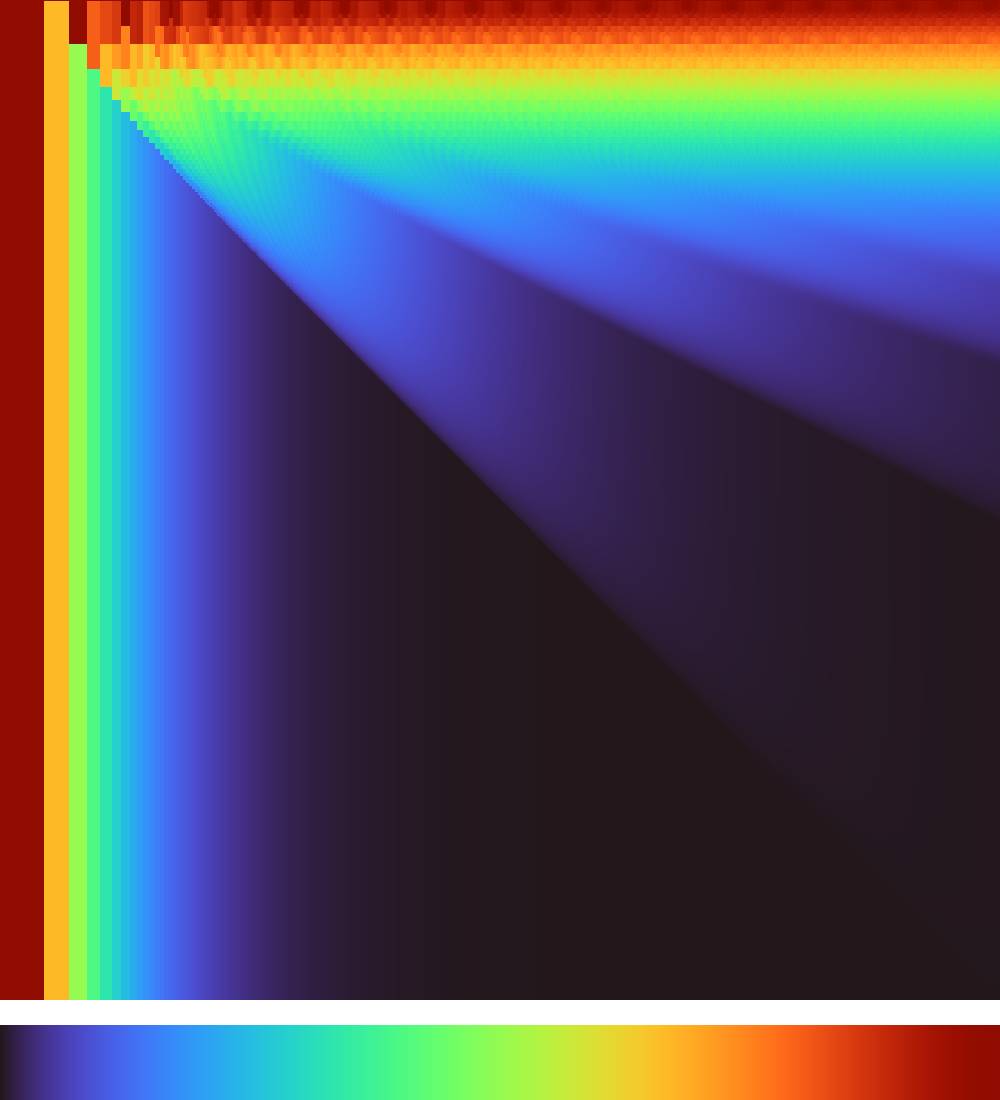
\includegraphics[scale=0.4]{w.png}\,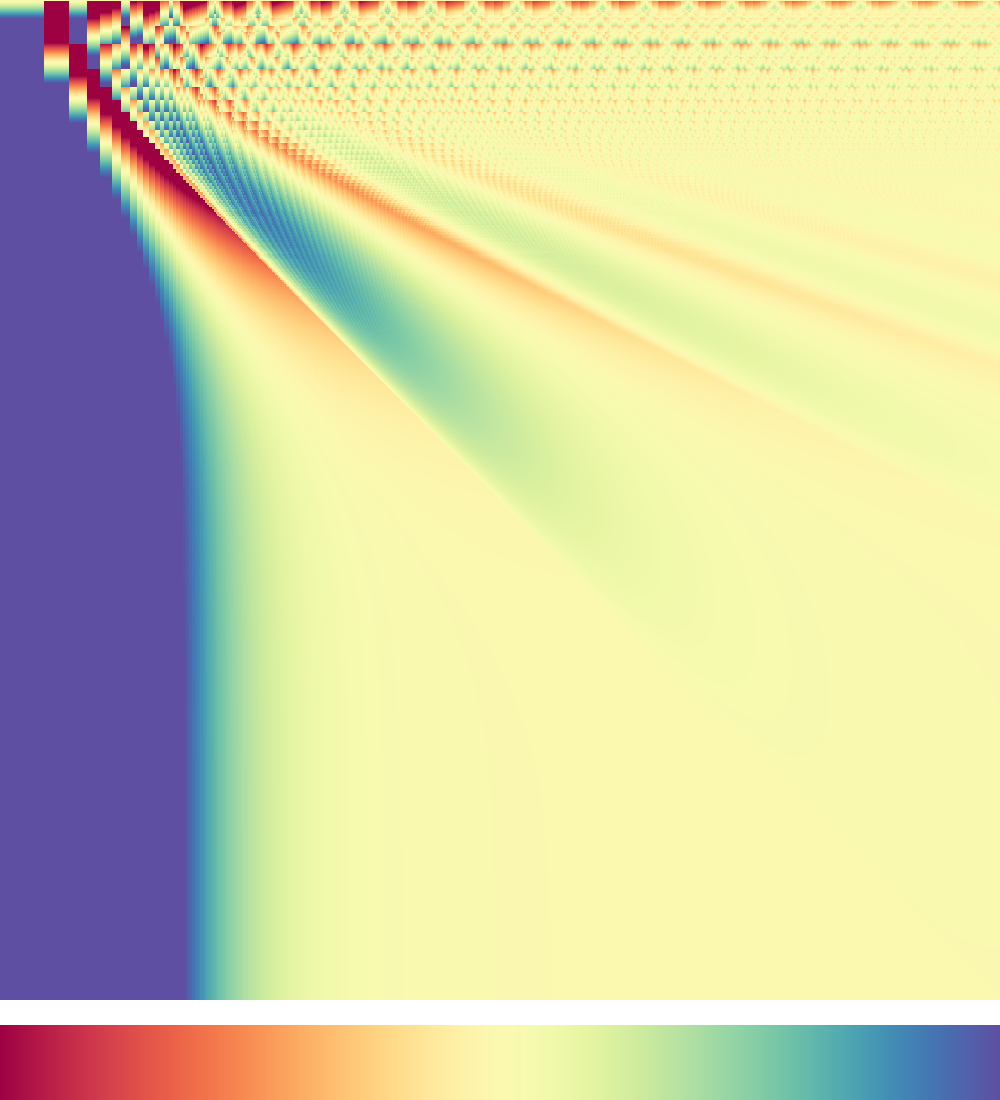
\includegraphics[scale=0.4]{bias.png}
	
	\hspace{1cm}
	
	
\includegraphics[scale=0.4]{variance.png}\,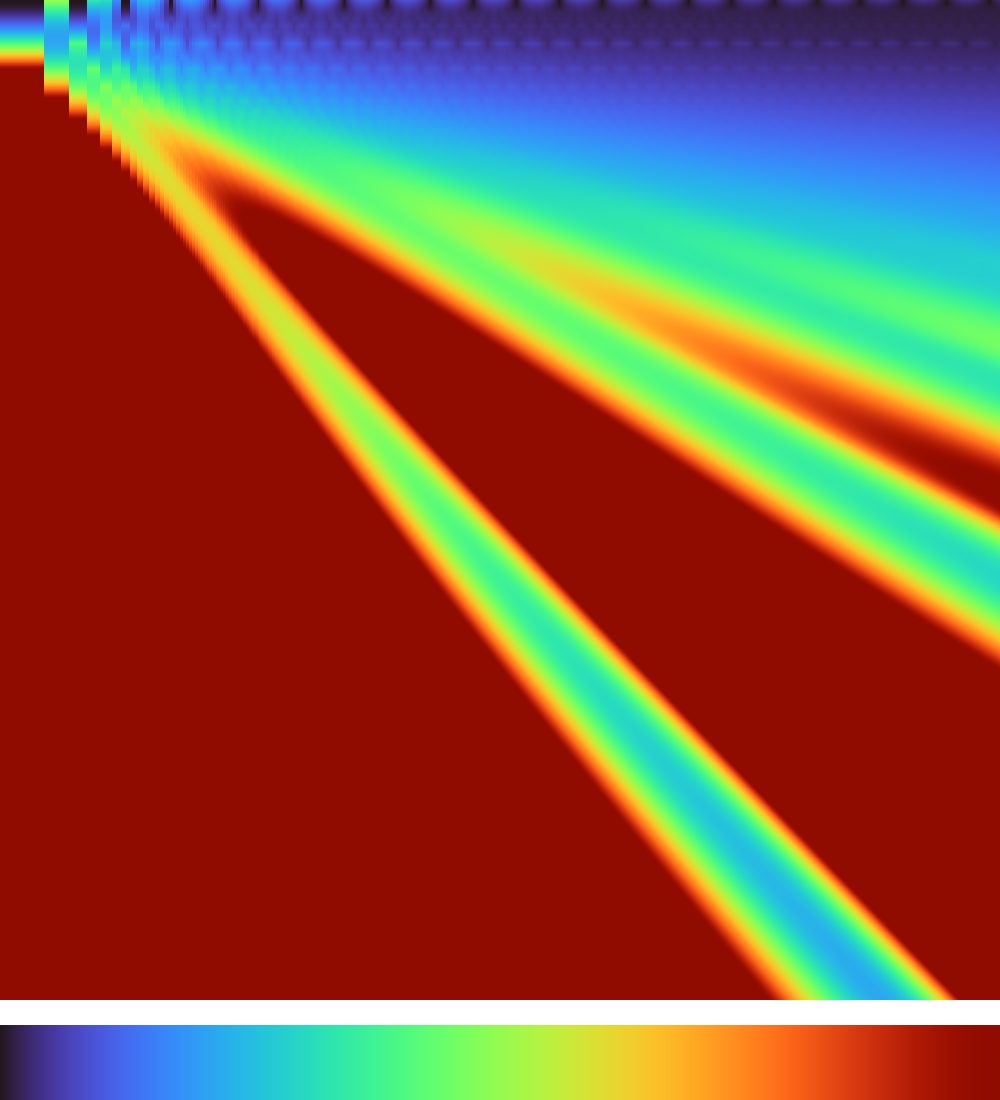
\includegraphics[scale=0.4]{e-bias.png}
	
	\hspace{1cm}
	
	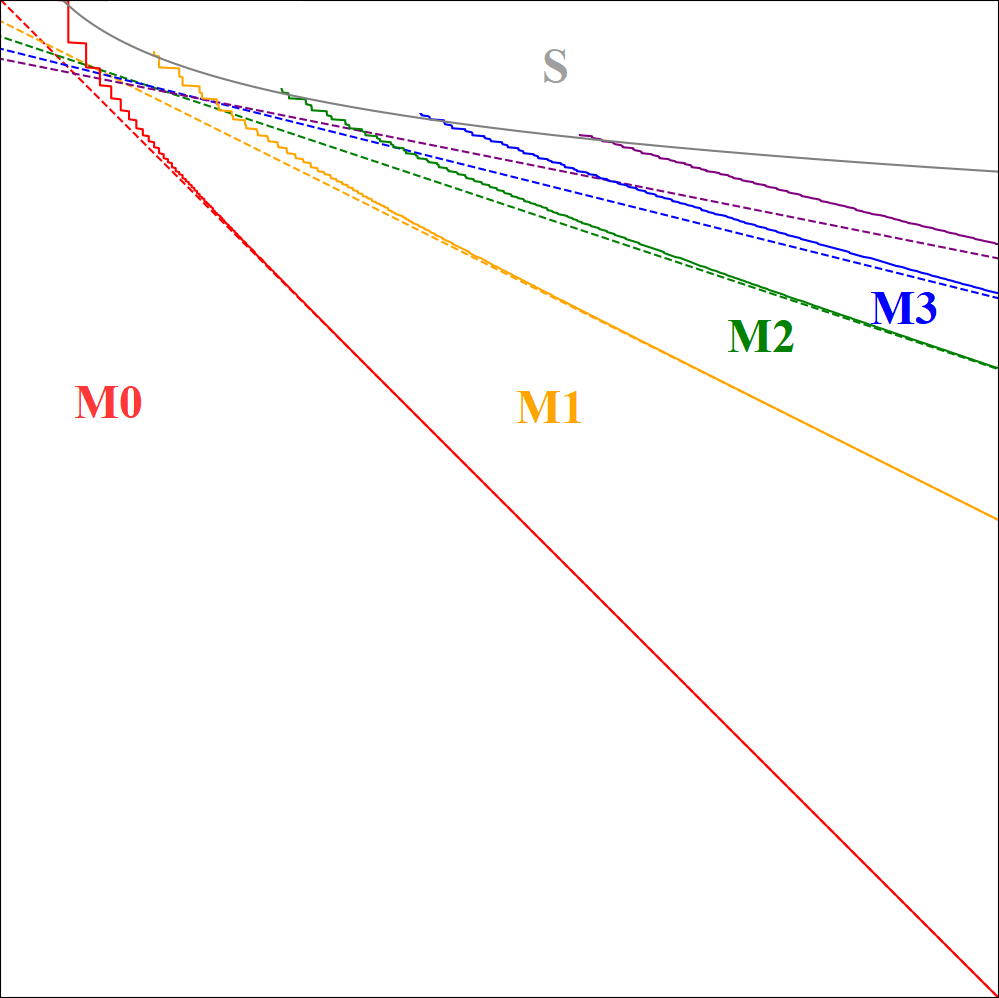
\includegraphics[scale=0.4]{mode.png}
	
	The first graph id colored using the average relative optimizer $w_{s,t}(n)$, where color gradients runs from 0.0 to 0.5
	\[
	c_1 = \frac{w^{max}_{s,t}(n) + w^{min}_{s,t}(n)}{2n}
	\]
	The second graph is colored using the relative difference of optimizer $w_{s,t}(n)$ against the continuous optimizer, where 0 difference is light yellow:
	\[
	c_2 = \frac{w^{max}_{s,t}(n) + w^{min}_{s,t}(n)}{2n} - g_{s,t}
	\]  
	The third graph is colored using the relative variance of optimizer $w_{s,t}(n)$, where 0 is colored dark green
	\[
	c_3 = \frac{w^{max}_{s,t}(n) - w^{min}_{s,t}(n)}{n}
	\]
	The forth graph is colored using the relative difference between $E(n)$ and its continuous version, where dark blue means little difference, while dark red means $E(n)$ is significantly higher
	\[
	c_4 =\frac{E_{s,t}(n)} {\tilde{E}_{s,t}(n)} = \frac{E_{s,t}(n)} {k_{s,t} n \ln n}
	\]
	We can see the graph is divided into several regions. We have already discussed mode $M_0$ and $M_1$ above. There are also mode $M_2$, $M_3$ and so on. A new mode $M_{n+1}$ is formed when the ``short branch" ($E(w)$ when $w$ is small) falls into mode $M_n$. For mode beyond $M_4$, they seems to ``fade away" and becomes very close to the continuous optimizer.
	
	Around $s \approx t$, there is mode $S$.
\end{proof}

%%%%%%%%%%%%%%%%%%%%%%%%%%%%%%%%%%%%%%%%%%%%%%%%%%%%%%%%%%%%%%%%%%%%%%%%%%%%%%%%%%%%%%%%%%%%%%%%%%%%%%%


\section{Back to the classic binary search}
In the original binary search problem is represented by $s = t = T$. In this case, the recursive equation becomes
\[
F_{s,t}(n) = T + \min_{0<w<n}\left\{\frac{w}{n}F_{s,t}(w) + \frac{n-w}{n}F_{s,t}(n-w)\right\}
\]

TODO



\end{document}